The goal of this chapter is to give a description of the \textit{Bacco} protocol and to discuss the
implementation choices that were made in order to deploy it. This is achieved using a top-down ordering for the level
of detail, meaning that an overview of the network is presented before the specifics of the MAC protocol.

\section{Network overview}
I will start by describing a simple network that makes use of the protocol to better understand the integration of the
Bacco protocol into an LPWAN. The network is built upon 4 categories of devices:

\begin{description}[font=$\bullet$~\normalfont\scshape\color{blue!50!black}]
    \item [Sender node] - collects data and sends it to the gateway using LoRa
    \item [Repeater node] - listens to the incoming LoRa messages form Senders and sends them to a Gateway \footnote{The use of Repeaters where
            physical obstacles compromise the integrity of the signals is of very high
        relevance in agricultural contexts, since natural barriers such as hills can easily block \gls{VHF} radio signals.}
    \item [Gateway node] - collects data coming from the sender nodes and sends it to the web server. In the example
        shown, this will be achieved with the FTP protocol over a mobile network such as \gls{GSM} or \gls{LTE}. This node has
        also the role of coorinating and syncronizing Sender nodes. It can also be optionally configured to perform pre-processing operations (e.g.\ filtering, smoothing, interpolation ...) on the incoming data
    \item [Web server] - receives data coming from the Gateways, elaborates it and makes it available
        through a web application
\end{description}

\begin{figure}[ht]
    \centering
    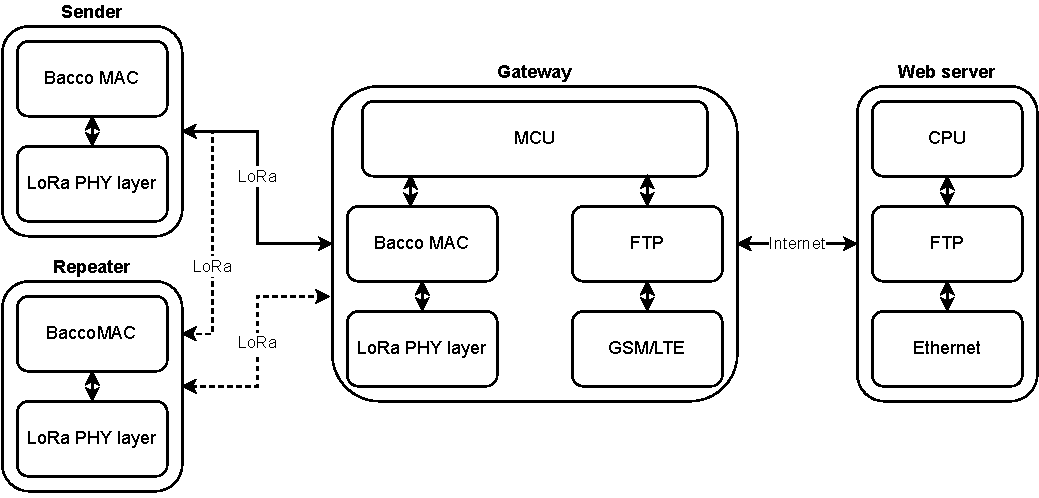
\includegraphics[width=1.0\textwidth]{uml/network_stack.pdf}
    \caption{Schematic representation of the example network}
    \label{network stack img}
\end{figure}

\section{Topology}
The network has a star-of-stars topology, in which the zeroth level is occupied by the Web server, the first level by the
Gateways and Repeaters, and the second level contains the Senders.
Figure \ref{network topology img} shows the type of devices that are involved and their communication schema. \\
The structure is equivalent to a tree, hence we can define a hierarchy of nodes. The root node is the central web server
and its children nodes are the Gateways. All sender nodes are children of either a Gateway or a Repeater and have to
chlidren, so they correspond to the leaves of the tree.

\begin{figure}[ht]
    \centering
    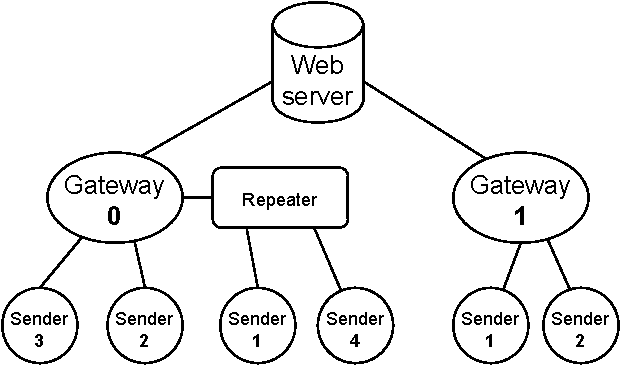
\includegraphics[width=1.0\linewidth]{uml/network_topology.pdf}
    \caption{Example network topology}
    \label{network topology img}
\end{figure}

\section{Addressing}
It is crucial to identify each Sender node in order to contextualize the messages coming to the Gateway node.
This is achieved by assigning them a unique identifier, represented by a natural number in the range $\[1,254\]$.
Address 0 is reserved for the Receiver and address 255 is used as a globally invalid address.
This fact limits the number of Sender nodes connected to a single Gateway to 254 \footnote{This choice is influenced
by the current Italian regulations \colorbox{red}{TODO: Scrivi e inserisci citazione a paragrafo su regolamentazione e
calcolo numero massumo di devices} \cite{CITAZIONE PARAGRAFO REGOLAMENTAZIONE E CALCOLO MASSIMO NUMERO DI DEVICES} \cite{gazzetta_potenza_868} on duty cycle for the 868MHz band and the fact that most agricultural contexts do not require a huge amount of sensors}. If necessary, the network can scale up by using additional Gateways.
Note that since Repeaters do not modify the forwarded messages and do not produce messages themselves, they do not play
an active role in the network and thus they will not be given an identifier.

\section{Interference mitigation}
The LoRa PHY protocol specification does not fully cover the matter of sharing the communication link between multiple
devices, thus it is necessary to define mothods for doing so, in order to minimize interference and achieve
a realiable exchange of information. Different techniques are applied in the domain of both time and frequency

\subsection{Channel activity detection}
Channel Activity Detection, or CAD, is a feature available for most LoRa transcievers\cite{cad}. In this mode, the LoRa node
listens for any transmission on a specific frequency; if it detects a signal, it retuns an interrupt to the MCU. This
presents a possible Carrier Sense Multiple Access mechanism, also called CSMA.\\
Bacco does not make use of CAD for data packets, but it enables it in specific situations such as network discovery (discussed
in section \ref{Network discovery}).

\subsection{IQ inversion}
IQ inversion is a LoRa primitive that makes it possible to have 2 types of transmissions on the same frequency and
spreading factor that are easily
distinguishable for a receiver. The name stands for \emph{In-phase / Quadrature}, and it usually refers to
signals that are out of phase from each other by $\frac{\pi}{4}$ rad. Despite of that, LoRa uses that term to describe
2 signal with inverted chirp direction, namely up-chirp and down-chirp (see figure \ref{img: iq inversion}). Bacco uses this technique to discriminate between uplink messages (i.e. from Sender to
Gateway/Repeater) and downlink messages (i.e. from Gateway to Sender/Repeater). This implies that devices belonging to
the same category are not able to communicate with each other (e.g. a Sender would not detect other Senders' transmissions).

\begin{figure}
    \centering
    \begin{subfigure}[b]{0.45\linewidth}
        \begin{subfigure}[b]{\linewidth}
            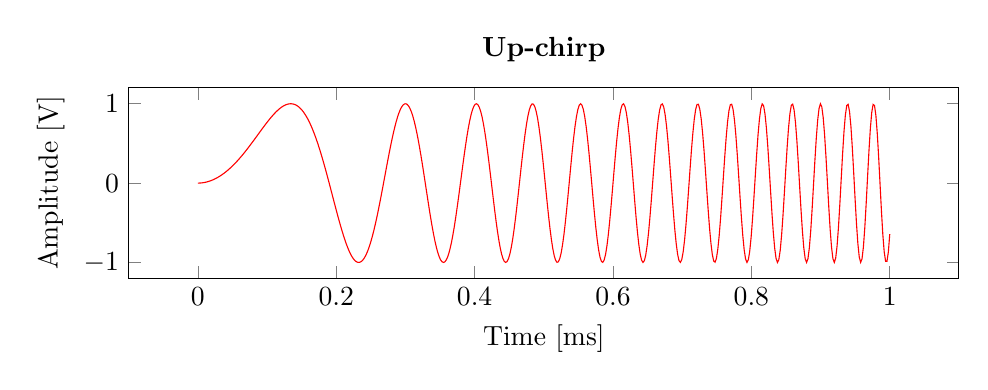
\begin{tikzpicture}
                \begin{axis}[width=\linewidth, height=4cm, title={\textbf{Up-chirp}}, xlabel={Time [ms]}, ylabel={Amplitude [V]}]
                    \addplot[color=red, samples=500][domain=0:1]{sin(x*x*5000)};
                \end{axis}
            \end{tikzpicture}
        \end{subfigure}
        \begin{subfigure}[b]{\linewidth}
            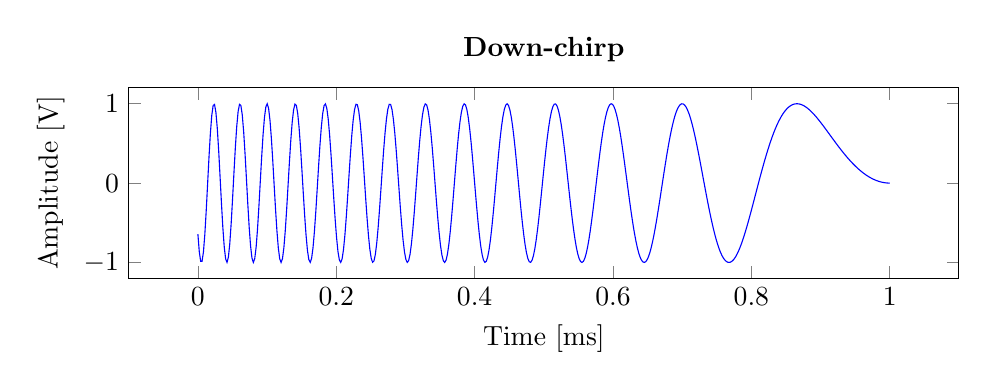
\begin{tikzpicture}
                \begin{axis}[width=\linewidth, height=4cm, title={\textbf{Down-chirp}}, xlabel={Time [ms]}, ylabel={Amplitude [V]}]
                    \addplot[color=blue, samples=500][domain=0:1]{sin(5000*(1-x)*(1-x))};
                \end{axis}
            \end{tikzpicture}
        \end{subfigure}
    \end{subfigure}
    \hspace{0.08\linewidth}
    \begin{subfigure}[b]{0.45\linewidth}
        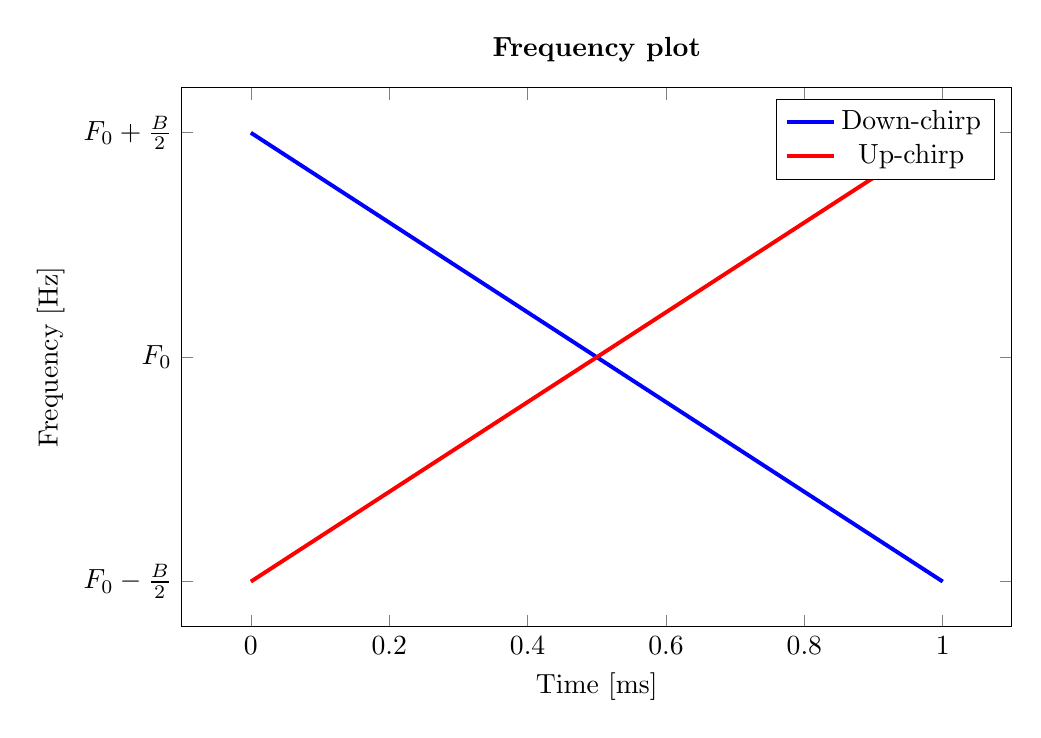
\begin{tikzpicture}
            \begin{axis}[width=\linewidth, height=8cm + \baselineskip, title={\textbf{Frequency plot}}, xlabel={Time
                [ms]}, ylabel={Frequency [Hz]}, ytick={0, 0.5, 1}, yticklabels={$F_0-\frac{B}{2}$, $F_0$, $F_0+\frac{B}
                {2}$}, legend entries={Down-chirp, Up-chirp}]
                \addplot[line width=0.5mm, color=blue, samples=500][domain=0:1]{1-x};
                \addplot[line width=0.5mm, color=red, samples=500][domain=0:1]{x};
            \end{axis}
        \end{tikzpicture}
    \end{subfigure}
    \label{img: iq inversion}
    \caption{IQ inversion}
\end{figure}

\subsection{Subnetting}
The LoRa procol supports a wide range of carrier frequencies in the \gls{VHF} spectrum \footnote{For reference, the
SX1262\cite{sx1262} transciever features a continuous frequency coverage from 150 MHz to 960 MHz}. This feature makes
it possible to apply various techniques to mitigate interference.\\
Bacco exploits it to build sub-networks that operate at different frequencies, and thus achieve a communication with very low
interference between different sub-nets. Specifically, all the Sender nodes connected to a Repeater and the Repeater
itself operate at a frequency that's different from the frequency used by the Gateway and other Repeaters. Figure \ref{repeaters
subnet} shows a schematic representation. This technique is particularly useful to solve the problem of bouncing, that occours
when a message is sent back to the original Repeater.\\
It is necessary to define a set of frequencies at which Repeaters and Gateways operate. This choice is done
based on current regulations in the specific country of operation; this thesis will focus on Italian and/or European
standards. 868 MHz is the base frequency at which the Gateway node operates, and the set of 6 frequencies of operation
is so composed:
\begin{equation}
\label{set of frequencies}
\left\{ f_k : f_k = 868\text{MHz} + k \times 125\text{KHz}, k\in \left\{0..10 \right\} \right\}
\end{equation}
This implies that a Bacco network can have up to 10 Repeaters operating on different frequencies, however if more coverage
is needed, it is possible to have multiple Repeater nodes working at the same frequency, given that they are not in
reach with each other.


\begin{figure}[ht]
    \centering
    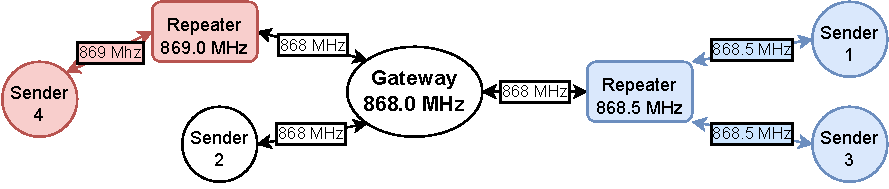
\includegraphics[width=\linewidth]{uml/repeaters_subnet.pdf}
    \caption{Example network with repeaters in subnets}
    \label{repeaters subnet}
\end{figure}


\subsection{Distribution of transmission activity}
The Bacco protocol distributes the activity on the channel over time using defined frames reserved for each Sender, using
an approach that was first introduced by the AlohaNet\cite{alohanet} protocol. The frames are equally distributed between
all the Senders and the start of each transmission frame is function of the identifier. The time delay between 2 consecutive
transmissions from a same Sender is a constant value and it is called cycle. At the end of a cycle, some time is
reserved for the Gateway to upload the collected data. Figure \ref{timing diagram} shows a schematic representation of
the time slot management used by Bacco. The cycle time is a user-defined parameter, and all the other values are
calculated based on it as shown in table \ref{timing table}. \\

\begin{table}[ht]
    \centering
    \setlength{\extrarowheight}{5pt}
    \begin{tabular}{ |c|c| }
        \hline
        \textbf{Parameter} & \textbf{Value}\\
        \hline
        Gateway frame time & $0.2 \cdot C$\\
        \hline
        Sender frame time & $\frac{0.6 \cdot C}{N}$\\
        \hline
        Silence frame time & $\frac{0.2 \cdot C}{N}$\\
        \hline
    \end{tabular}
    \caption{Time parameters calculation, where C is the cycle time and N is the number of Senders}
    \label{timing table}
\end{table}

\begin{sidewaysfigure}
    \centering
    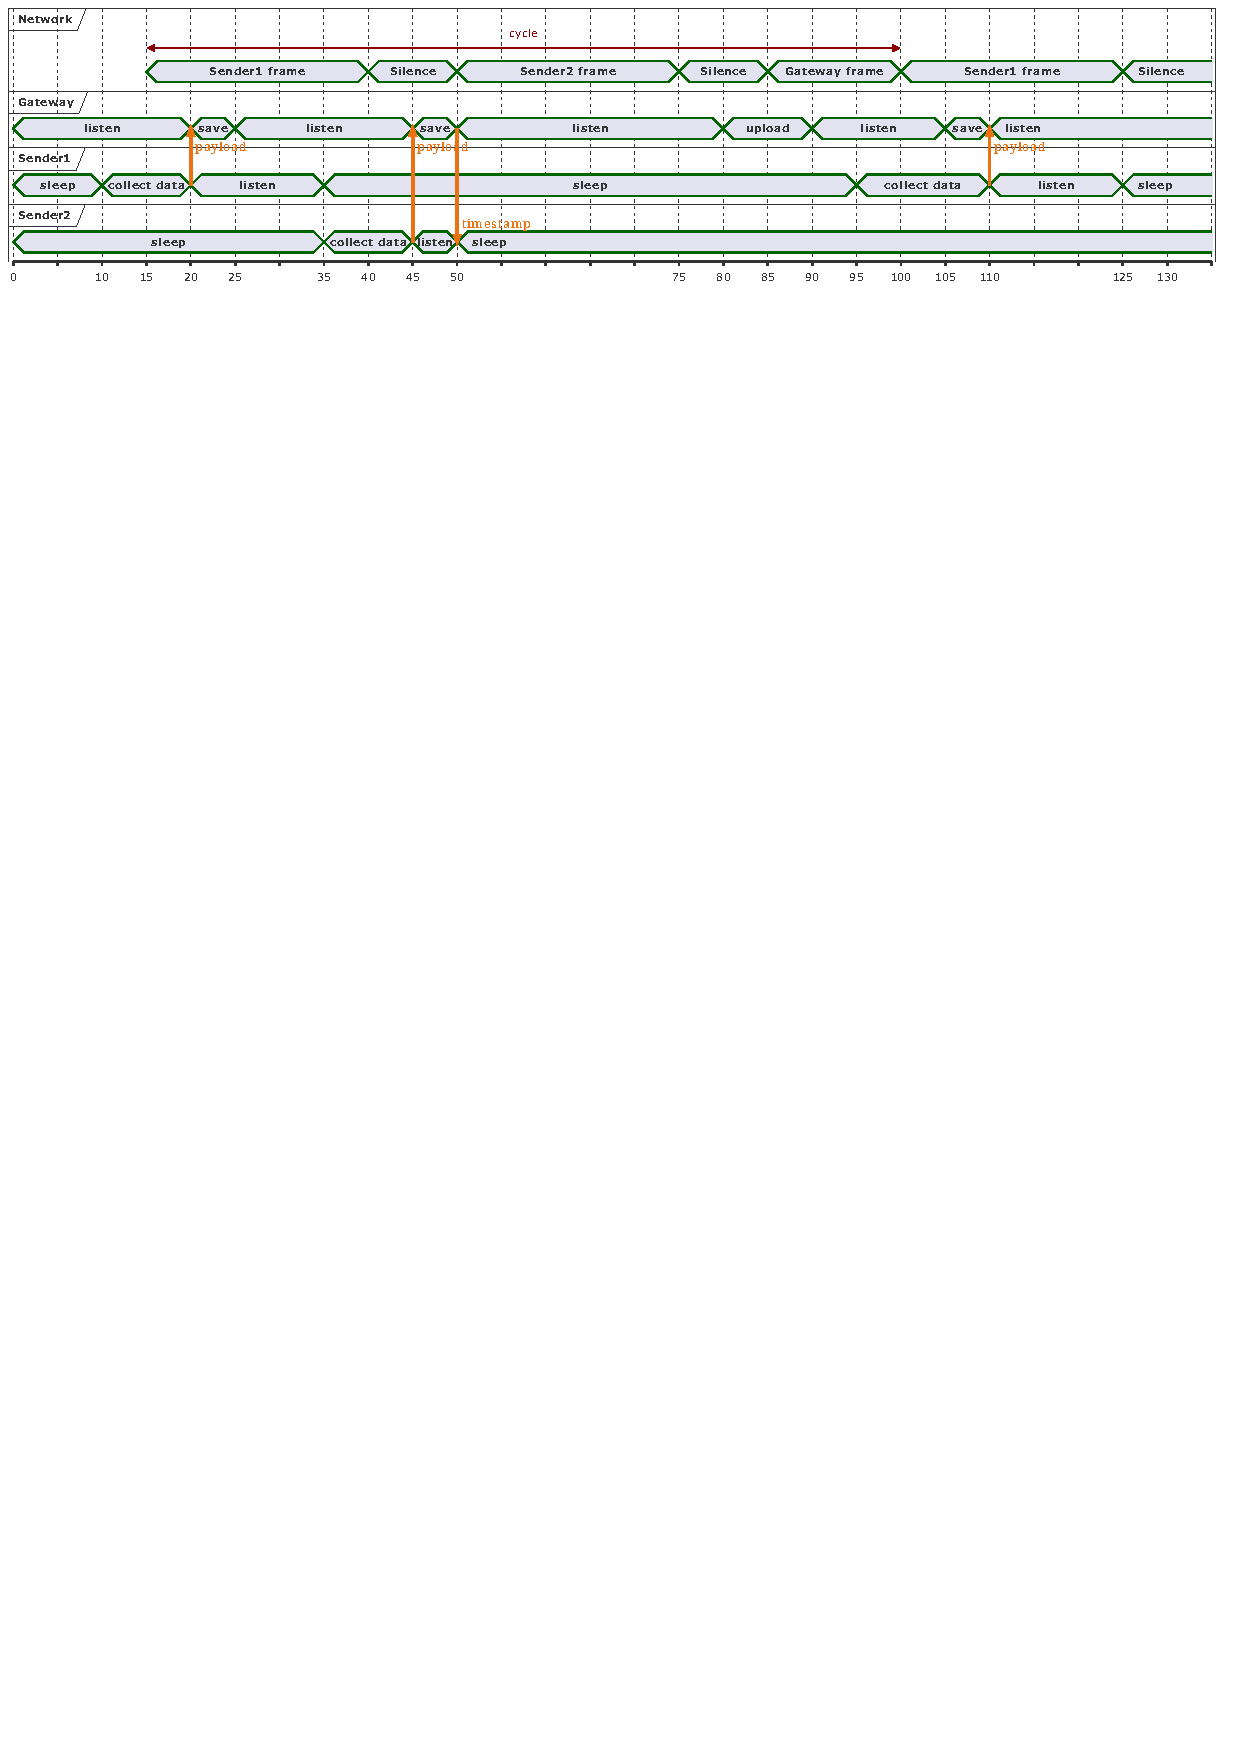
\includegraphics[clip, trim=0cm 25.2cm 0cm 0cm, width=1.0\textwidth]{uml/timings.pdf}
    \caption{Timing diagram}
    \label{timing diagram}
\end{sidewaysfigure}

\subsubsection{Compensating clock drift}
All the devices in the network need to transmit during their assigned frame for the protocol to be effective; this means
that all the clocks are required to have a certain degree of syncronization. This is hard to achieve in
practice, because all commercial clock oscillators do not provide a costant frequency source due to manifacturing imprecisions,
temperature gradient etc... .\\
In order to deal with with this problem, Bacco assigns the Gateway node the role of coordinating the network timings through
the dispatch of downlink messages containing the network timestamp when a Sender
node transmits out of its assigned frame. The downlink message is sent as soon as the Gateway receives the uplink
message. Figure \ref{timing diagram} shows this behavior during the transmission involving Sender2.
The Gateway sends at least one downlink message every 10 uplink messages from a same Sender, to ensure syncing and to
signal that the connection is still active.

\section{Network discovery}
\label{Network discovery}
When a Sender node is first started, it needs to decide at what frequency it has to operate for minimizing the power
needed to reach a Repeater or Gateway. In order to do this, Bacco introduces method \ref{algo:network discovery}
for scanning nearby devices and selecting the most suitable. It tries to establish a communication with Repeaters and
Gateways spanning all the available frequencies by sending a particular type of message that triggers a response
containing a SYN/ACK message. Note that the CAD technique will be used by the Sender to not interfere with ongoing
communications because the board does not yet have an allocated time frame.

\begin{algorithm}
    \caption{Network discovery algorithm}\label{algo:network discovery}
    \begin{algorithmic}

        \State rssi\_values $\gets$ $\[0,0,0,0,0,0,0,0,0,0\]$

        \While{all rssi\_values are equal to 0}
            \For{$k$ from 0 to 10}
                \State $f_k$ $\gets$ $868 \times 10^6 + k \times 125 * 10^3$
                \For{$i$ from 0 to 10}
                    \Do
                        \State sleep for 1 second
                        \State enter CAD mode at frequency $f_k$ for 1.5 seconds
                    \doWhile{activity detected by CAD}
                    \State send sensing message
                    \State enter receive mode for 3 seconds
                    \If{received SYN/ACK}
                        \State $\text{rssi}\_values\[k\]$ $\gets$ current rssi
                        \State \textbf{break}
                    \EndIf
                \EndFor
            \EndFor
        \EndWhile
    \end{algorithmic}
\end{algorithm}


\section{Network joining}
When a Sender node needs to connect to a Gateway node for the first time, it does not yet have an identifier nor is in
sync with the network. The procedure to achieve that will be called the joining process. Note that we assume that the
Sender node has already selected its frequency of operation, as descibed in section \ref{Network discovery}.\\
We will ignore the act of forwarding made by any optional Repeater node, as in this case is transparent for both ends of the
communication. All the messages sent from Sender and Receiver make use of CAD to make sure the channel is free before
the actual transmission; this step will be omitted in the description for brevity. First, the Sender transmits a SYN
message to the Gateway and waits for a SYN/ACK response for 3 seconds. If no message is received, another SYN message
is sent for a maximum of 10 times. After that, the Gateway waits for 3 seconds for an ACK message from the Receiver, and
if no message is received it will try again for a maximum of 10 times. The SYN/ACK message contains the timestamp of
the network as well as the assigned identifier. If the maximum number of iterations are reached in any of the steps, the
whloe process starts again after 30 minutes. Figure \ref{img: network joining} show a schematic representation of the process.

\begin{figure}[ht]
    \centering
    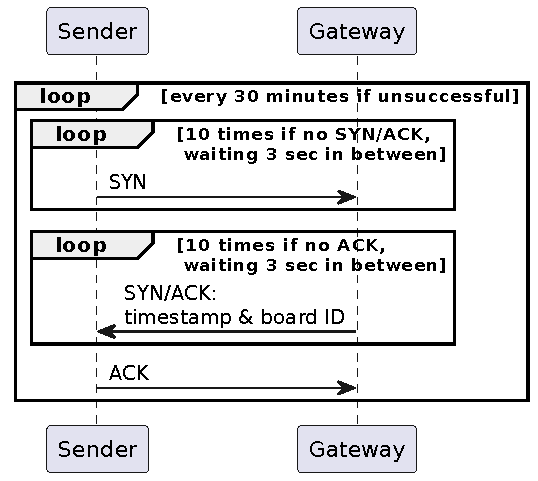
\includegraphics[width=200pt]{uml/network_joining.pdf}
    \caption{Network joining process}
    \label{img: network joining}
\end{figure}

\section{Downlink commands}
In some situations (e.g. \ref{sec: transmission power adaption}), it is required to be able to change the behavior of the
network dynamically and in a reliable way. Bacco achieves this by exhanging specialized kind of packets that contain a
command. Each command message needs to be acknowledged by the Sender to the Gateway/Repeater in a similar way as done during the
network joining procedure. Figure \ref{img: command ack} offers a graphical representation. Every command is associated
to an opcode, as shown in table \ref{tab: opcodes}.\\

The following commands are defined by the protocol:
\begin{description}[font=$\bullet$~\normalfont\scshape\color{blue!50!black}]
    \item [Shutdown] - If this command is sent and processed successfully, the Sender goes to sleep indefinetly until a manual reset is invoked by physically pressing a button
    \item [Enter quiescent mode] - If this command is sent and processed successfully, the Sender stops to send data, but it keeps
        listening during its time frame
    \item [Wakeup from quiescent mode] - If this command is sent and processed successfully, the Sender enters normal/active mode
        and thus starts to transmit data again
    \item [Increase transmission power] - If this command is sent and processed successfully, the Sender increases its
        transmit power by 3dBm
    \item [Decrease transmission power] - If this command is sent and processed successfully, the Sender deceases its
        transmit power by 3dBm
\end{description}

\begin{table}[ht]
    \centering
    %\setlength{\extrarowheight}{5pt}
    \begin{tabular}{ |c|c| }
        \hline
        \textbf{Command} & \textbf{Opcode as unsigned integer}\\
        \hline
        Shutdown & 0\\
        \hline
        Enter quiscent mode & 1\\
        \hline
        Wakeup from quiescent mode & 2\\
        \hline
        Increase transmission power & 3\\
        \hline
        Decrease transmission power & 4\\
        \hline
        Reserved for later use & [4-50]\\
        \hline
        User defined & [51-127]\\
        \hline
    \end{tabular}
    \caption{Table of opcodes}
    \label{tab: opcodes}
\end{table}

\begin{figure}[ht]
    \centering
    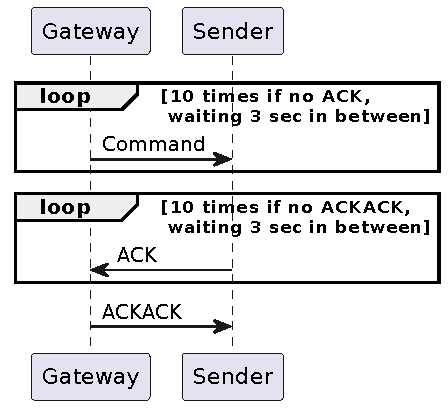
\includegraphics[width=200pt]{uml/command_ack.pdf}
    \caption{Command sending process}
    \label{img: command ack}
\end{figure}

\section{Transmission power adaption}
\label{sec: transmission power adaption}
Since Senders can be placed at different distances from a Gateway or Repeater, it is useful to optimize the power
used by the node to transmit. The default value for the transmission power is equal to $P_{0}$; starting from that, the
network will automatically drift towards a more suitable value according to the
following triggers:
\begin{itemize}
    \item If on the Sender side, the device has not received any downlink messages during
        the last 20 frames belonging to it, then \textbf{increase TX power} by $P_{step}$
    \item If on the recevier side (either Repeater or Gateway), all the last 10 transmission
        satisfy $\text{RSSI} < \text{RSSI}_{high}$ and $\text{SNR} < \text{SNR}_{high}$ or have not been received, then
        send a command message to the Sender telling to \textbf{decrease TX power} by $P_{step}$
    \item If on the recevier side (either Repeater or Gateway), all the last 10 transmission
        satisfy $\text{RSSI} > \text{RSSI}_{high}$, then send a command message to the Sender telling to
        \textbf{decrease TX power} by $P_{step}$.
\end{itemize}
Here the parameters are shown:
\begin{equation}
    \begin{array}{l}
        P_{0} = P_{max} = 14\text{ dBm} \\ P_{step} = 3\text{ dBm} \\ \text{RSSI}_{low} = -115\text{ dBm} \\ \text{RSSI}
        _{high} = -60\text{ dBm} \\ \text{SNR}_{low} = -7\text{ dBm}
    \end{array}
\end{equation}
Gateways and Repeaters always operate at $P_{0}$, since power efficiency is less critical than reliability for such nodes.


\section{Packet format}
In this section the bit format of the messages is shown. The analysis will be split in uplink packets and downlink
packets.

\subsubsection{Uplink packet format}
An uplink message is sent from a Sender to the Gateway, and can be optionally repeated by a Repeater. It has a variable
length and it is transmitted using up-chirps, i.e without IQ inversion enabled. Figure \ref{img: uplink packet format} shows its
format.

\begin{figure}
    \centering
    \begin{bytefield}[]{32}
        \bitheader{0,8,16} \\
        \bitbox{8}{Sender ID} & \bitbox{8}{Payload size}
                              & \bitbox{16}{Payload}
    \end{bytefield}
    \caption{Uplink packet format}
    \label{img: uplink packet format}
\end{figure}


\subsubsection{Downlink packet format}
A downlink message is sent from the Gateway to a Sender, and can be optionally repeated by a Repeater. It has a fixed
length of 5 bytes and it is transmitted using down-chirps, i.e with IQ inversion enabled. Figure \ref{img: downlink
packet format}, \ref{img: downlink timestamp packet format}, \ref{img: downlink commmand packet format} show its format.

\newcommand{\bitlabel}[2]{%
    \bitbox[]{#1}{%
        \raisebox{0pt}[4ex][0pt]{%
            \turnbox{65}{\fontsize{9}{9}\selectfont#2}%
        }%
    }%
}
\begin{figure}
    \centering
    \begin{bytefield}[]{40}
        \bitlabel{8}{} & \bitlabel{1}{Message type} & \bitlabel{31}{}\\
        \bitheader{0,8,9,39} \\
        \bitbox{8}{Sender ID} & \bitbox{1}{}
                              & \bitbox{31}{Payload}
    \end{bytefield}
    \caption{Downlink packet format}
    \label{img: downlink packet format}
\end{figure}

\begin{figure}
    \centering
    \begin{bytefield}[]{40}
        \bitheader{0,8,9,39} \\
        \bitbox{8}{Sender ID} & \bitbox{1}{0}
                              & \bitbox{31}{Timestamp}
    \end{bytefield}
    \caption{Downlunk timestamp packet format}
    \label{img: downlink timestamp packet format}
\end{figure}

\begin{figure}
    \centering
    \begin{bytefield}[]{40}
        \bitheader{0,8,9,39} \\
        \bitbox{8}{Sender ID} & \bitbox{1}{1}
                              & \bitbox{7}{Opcode}
                              & \bitbox{24}{Padding}
    \end{bytefield}
    \caption{Downlunk command packet format}
    \label{img: downlink command packet format}
\end{figure}
